\chapter{Method}\label{ch:Method}

\section{The dataset}

The dataset was the entire collection of every Reddit comment (including deleted comments) posted on December 2018. Due to the sheer size of the dataset being very hard to parse as one large dataset, it was decided to parse down comments to specific subreddits. (Table to be added in R)  The data was stored in the json format.

Each subreddit was placed its own json file and kept in cloud storage, allowing to be accessed by any of our team members. Each dataset has a varying level of bot created comments, which depends on how heavy the automated moderation is on each subreddit. To deal with this, we filtered out any users with a “-bot” suffix and any users that had a history of posting the the same type of comment repeatedly. An example of this would be AutoModerator, a popular bot used to automate moderation of subreddits. 

\section {Data preparation}
After clearing out the bot users, the data is further filtered out to only the required fields. The main ones used were Score, User, the content of the message, the date it was posted and the length of the message.

For text mining and processing. It was required to prepare the text of the comments for meaningful analysis. The first step was to remove common words and filter out “stop words” used in the English dictionary. Afterwards, the text was stemmed to reduce words to their core meaning. An example of this would be reducing “enhancing” just to “enhance”. 

Document term and term document matrices were created after the stemming process was completed, at this point it was possible to perform exploratory text analysis and to gain a better understanding of the vocabulary used by each subreddit community. This was done in order to prove that each subreddit provides a context which radically changes the vocabulary that each user uses.

\section {Basic Analysis}

\subsection {Relationship between original post time vs time since posted.}
	One of the vectors investigated was the relationship time has on the popularity of posts. Analysis shows that posts that are posted earlier are much more likely to get a higher score. The mean score goes down further on as time progresses before flat-lining at 100 5 minute intervals. Therefore, we can conclude that the mean score settles after 8.3 hours after the original post was created if you divide 500 minutes by 60.
	\begin{figure}[ht]
		\centering
			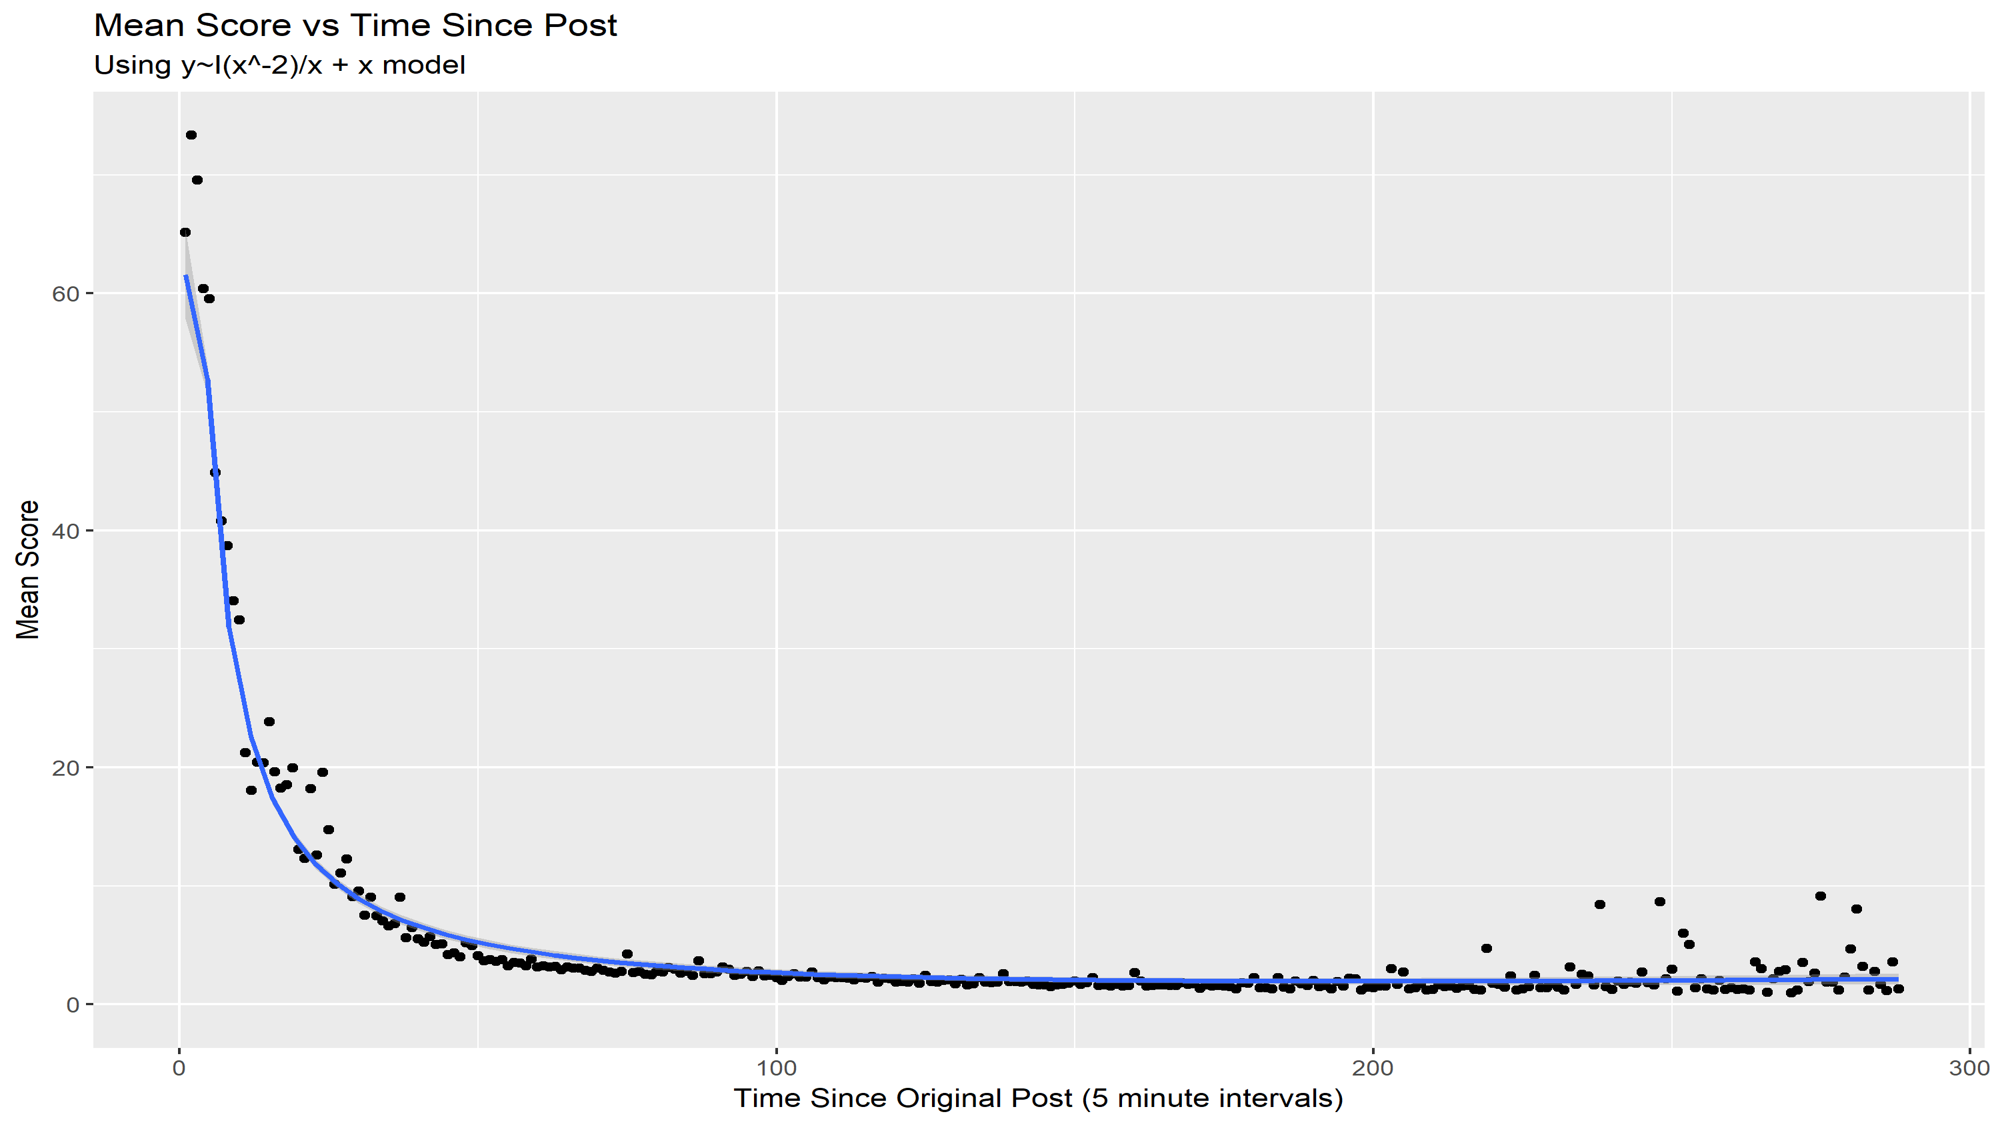
\includegraphics[width=1.0\textwidth]{graphs/meanscore_vs_time2}
		\caption{\textit{The time since the Original post was sent versus the mean score of every post within that 5 minute interval. Posts closer to post time tend to garner a much higher score. With this said, there is some outliers that begin to form near the tail end of the line. that beat the average.}}
	\end{figure}

\subsection{Relationship between length of comment and post score}
	This was tested to see if there was any correlation between the length of the comment measured in number of characters, vs the posts score which is an integer value. What we can see in the graph below is that there is no correlation between a posts score and the length of the comment. From this we can assume that a comments score is determined by the content of said comment, which is likely to vary from each subreddit. For example a posting a meme in /r/politics may not get the same reception that it would in /r/DankMemes as the subculture of politics orients itself to be for more serious conversations compared to /r/DankMemes which is all about humour.
	\begin{figure}[ht]
		\centering
			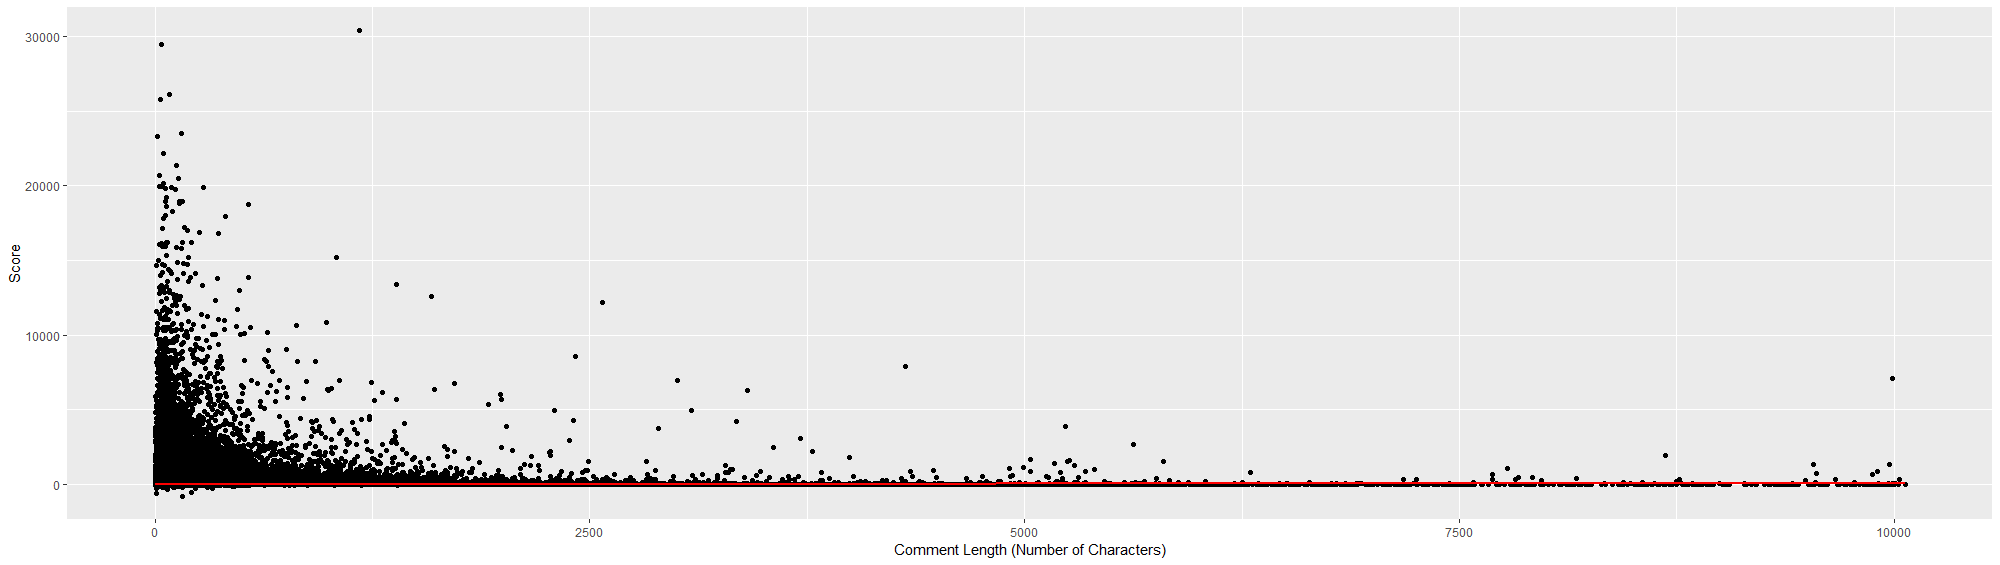
\includegraphics[width=1.0\textwidth]{graphs/length_score_all_subs}
		\caption{\textit{The length of a comment versus the mean score of all comments of that particular length}}
	\end{figure}




\section {Exploratory Text Analysis}


\section {Comment features}

\section {Machine learning experiment}



\section{Conclusions}




